\documentclass[12pt]{article}

\usepackage{amssymb,amsmath,amsfonts,eurosym,geometry,ulem,graphicx,caption,color,setspace,sectsty,comment,footmisc,pdflscape,subfigure,array,hyperref}
\usepackage{cite}
\usepackage{natbib}
\usepackage{etoolbox}
\usepackage{float}
\usepackage{algpseudocode}
\usepackage{booktabs}
\usepackage[font=footnotesize]{caption}

\AtBeginEnvironment{algorithm}{\setstretch{1}}

\normalem

\geometry{left=1.5in,right=1.5in,top=1.0in,bottom=1.0in}

\begin{document}

\begin{titlepage}
\title{Improving Dynamic Kidney Exchange}
\author{Vitor Hadad\thanks{Boston College}}
\date{December 2017}
\maketitle
\begin{abstract}

\bigskip
\end{abstract}
\setcounter{page}{0}
\thispagestyle{empty}
\end{titlepage}
\pagebreak 

%\doublespacing


\section{Introduction} \label{sec:introduction}


\paragraph{Main idea} We propose a new dynamic kidney matching algorithm that takes as input a pool of patient-donor pairs and computes, for each cycle that is currently available for matching, a probability that it should be chosen to be cleared today, as well as another probability indicating whether we should not match any more cycles. In order to get these probabilities, our algorithm first produces a prior distribution estimated by observing past choices made by an infeasible optimal algorithm, and then updates these priors with simulations. 

Our algorithm faces two main challenges. The first challenge is the input data representation, because the relevant information consists not only of the characteristics of each donor-patient pair, but also the underlying structure of their compatibility graph. For example, we need it to be the case that the same cycle will have different probabilities of being matched depending on what who are all the other patient-pairs in the graph, what characteristics they have, and how compatible their are to each other. Our solution to this obstacle involves using mapping the raw input data and the compatibility graph to points on the euclidean space, and then using these as regressors.

The second challenge is output data representation. As we said above, one of the components of the output is a joint probability distribution over each available cycle, indicating the likelihood that the cycle will be matched today. However, the number of available cycles will be different at each period, so we need an algorithm that is able to output probability distribution over a vector of variable length. In this paper, we experiment with a variety of neural network architectures for this task, and we note that recurrent neural networks provide the best performance.



\paragraph{Main results} We test our algorithm in a variety of data-generating processes that we call \emph{environments}. Each environment was inspired by previous work on dynamic kidney matching, and has different rules governing which patient-donor pairs are compatible or what are their relevant observable characteristics. In each environment, we compare the performance of our algorithm, as measured by the number of matched pairs within a long time period, to two benchmarks. The first one is an infeasible optimal algorithm (\texttt{OPT}) that knows exactly which patients will be come to the pool and how long their sojourn will be, and is therefore able to compute the maximal matching cardinality. Our second benchmark is \texttt{Myopic}, an algorithm that greedily matches and clears the maximal matching at each period, and is used a proxy to the algorithms that are being used in many real life kidney exchanges. Our results show that we were indeed able to improve upon \texttt{Myopic}, proving that indeed there might be potential gains to be made from taking dynamic issues into serious consideration. 

Our simulations show that there is a sizable performance gap between \texttt{Myopic} and \texttt{OPT}: for the parameter combinations we have tested, \texttt{Myopic} may match only about 75\% of the pairs that \texttt{Myopic} matches. In addition, this performance gap widens as we increase the number of maximum cycle length from 2 to 3. 

At the same time, we remark that even after our improvements, the gap between \texttt{Myopic} and \texttt{OPT} resists. Therefore, in this paper we also invite other researchers to consider alternative algorithms for dynamic kidney exchange, or produce theoretical upper bounds for them. We hope that the new methods proposed in this paper serve as further inspiration for the field.


\section{Background and literature review} \label{sec:literature}

Since its proposal in the medical literature over three decades ago by \cite{rapaport1986case}, kidney exchange has been the subject of a great deal of attention in the academic literature. Throughout the past twenty years, developments in microeconomic theory and operations research and have informed, reshaped and improved how living donor transplants are conducted in many countries. More recently, computer scientists have also started to focus on the production of better and faster algorithms for kidney exchange.

Since this paper sits in the intersection between matching theory and computational economics, and uses methods drawn from computer science and machine learning. Let us take a brief look at these fields in turn. 


\subsection{Kidney Exchange} \label{subsec:kidney}

\paragraph{Definitions} 

>HLA compatibility can also be defined in terms of
mismatch acceptability—mismatches in allosensitized
transplant candidates that result in a negative crossmatch
[74]. In this context, unacceptable mismatches are antigens
reacting with antibody detectable in the patient
sera, whereas acceptable mismatches are those with no
detectable antibody


\paragraph{Early years} In economics, the literature on kidney exchange is started by \cite{roth2004kidney}, who provided a kidney exchange mechanism inspired by the \emph{housing} problem studied in the literature of mechanism design as in \cite{shapley1974cores} and later \cite{abdulkadirouglu1999house}. While their mechanism had significant virtues as being strategy-proof and Pareto-efficient, it also relied on large number of exchanges being conducted simultaneously, and drew criticism for making assumptions about heterogeneous preferences over kidneys. Responding to these assessments, a subsequent work by \cite{roth2005pairwise} focused on logistically practical mechanisms that used only 2-way exchanges and also had patients indifferent over all compatible kidneys. In a later paper, \cite{roth2007efficient} demonstrated via simulations that allowing for 3-way exchanges in addition to 2-way exchanges could increase the cardinality of matched pairs by a great deal, but also showed that larger cycles would only bring about modest improvements.


\paragraph{Recent advances in static matching problems} In the second half of the oughties, both in academic literature and medical practice the focus began to shift from exchanges via cycles to exchanges emanating from \emph{non-directed donors} (NDD) -- altruistic donors who have no patient attached to them and are willing to donate their organs to anyone who would need it. Such exchanges yield a \emph{chain} of transplants that begins with the NDD and may either terminate with the last pair donating to a waitlist recipient in a kidney registry, or not terminate at all and have the last pair's donor await an opportunity to become a future living donor. The former kind was dubbed \emph{domino paired donation} by \cite{montgomery2006domino}, and all its transplants occur simultaneously. In the latter kind, transplants occur may staggeredly over several months, hence it was named \emph{non-simultaneous, extended, altruistic donor chain} by \cite{rees2009nonsimultaneous}.\footnote{On occasion, NEAD chains have also been called \emph{Never-ending altruistic donor chains}, as relayed by \cite[p.~235-6]{roth2015gets}.}

A significant amount of attention was devoted in the next years to these NEAD chains, including notably \cite{ashlagi2011nonsimultaneous} and \cite{ashlagi2012need}, whose results show that NEAD chains benefit highly sensitized patients in sparse pools of moderate size, because they decrease the need for simultaneous double-coincidence of wants in the exchange market. In fact, in recent years \cite{anderson2015finding} reported that ``NEAD chains are responsible for the majority of successful kidney transplants conducted via kidney exchange at both the [Allied for Paired Donation] and within other major exchange programs".

\paragraph{Dynamic kidney exchange} Meanwhile, a small subliterature started focusing on the problem of \emph{dynamic kidney exchange} that concerns this paper. In a seminal paper, \cite{unver2010dynamic} posited a continuous-time model where pairs arrive according to a Poisson arrival rate, enter the pool whenever their donor is incompatible with them, and from thereon suffer a constant cost of waiting Ünver was able to derive dynamic mechanism that depends produces optimal n-way exchanges by leveraging additional simplifying assumptions, including that pairs do not leave the pool unless they are matched, and that pairs within the pool are only blood-type incompatible. These assumptions render all pairs homogeneous, which dramatically decreases the dimension of the state space and allows for an easily interpretable solution.

\cite{ashlagi2013kidney} note that the graphs of real-life pools tend to be sparse and filled with pairs that are either easy or extremely hard to match. In order to model this particular feature, they postulate a sparse heterogeneous random graph model containing only two such types, and propose a greedy algorithm that waiting until there are a certain number of each type, and then matches as many as pairs as possible. In a different vein, \cite{akbarpour2017thickness} introduces a simple model of stochastically arrival and departure. In their setting, they show that greedy algorithms that cleverly explout the time to match can can perform close to infeasible optimal benchmarks, even if these algorithms are ignorant about the global structure of the graph.

In the computer science and operations research literature, \cite{abraham2007clearing} and more recently \cite{anderson2015finding}, \cite{dickerson2016position} and \cite{dickerson2017small} have focused on producing scalable combinatorial programming algorithms that can take on tatic matching problems with large graphs and allowing for both chains and cycles of moderately large length. However, a series of papers starting with \cite{awasthi2009online} and followed by \cite{dickerson2012dynamic} and \cite{dickerson2015futurematch} have dealt with the dynamic kidney problem by \emph{weighted myopia}. Their idea is to prevent wasteful matchings (e.g., an O-donor to an AB-patient) by artificially introducing negative weights to graph components containing them. In \cite{dickerson2015futurematch}, these optimal weights are computed from simulations involving historical data.


\paragraph{Miscellaneous} Kidney exchange is a rich problem that can be studied from several different angles. For example, it is a special case of barter exchange, [[[Barter]]].  [[[Hospital incentives]]] [[[Medical literature]]]



\subsection{Machine learning and Artificial Intelligence}



\subsubsection{Neural Networks}

Neural networks are created by composing simpler parametric building blocks such as linear functions and simple nonlinear ones\cite{goodfellow2016deep}. Although they have existed for more than a half-century, in recent years they have received an enormous amount of attention in the statistical, computer science and optimization literatures. In this work, we will use \emph{multilayer feedforward networks}, \emph{recurrent neural networks} (with and without an extra property named \emph{attention}) and \emph{graph convolutional networks}. While a comprehensive survey on the motivation and use-cases of all these types of neural networks is outside the scope of this work, in the next paragraphs we will give an abridged overview of their definition and their immediate application to our problem. 

\paragraph{Feedforward Neural Networks} Also called \emph{multilayer perceptrons}, these functions process each input



\paragraph{Recurrent Neural Networks and Sequence-to-sequence models}
\paragraph{Embedding non-euclidean domains} \label{par:embedding}
\subsubsection{Search algorithms}



\section{Models, Environments and Data} \label{sec:data}

A \textbf{dynamic kidney exchange problem} is a discrete-time Markov Decision Process (MDP) described by the tuple $(S, A, P, R)$, where

\begin{itemize}
  \item $S = (V, A, X)$ is a directed graph representing the current \emph{state}: the set $V$ is the finite set of patient-donor pairs and their observable characteristics; and an adjacency matrix $A$ whose entry $(i,j)$ is positive whenever the donor of vertex $i$ can donate to the patient of vertex $j$. The set $X$ is a set of 
  \item $Act$ is the finite set of available \emph{actions} when the current state is $S$. In our applications, this is the set of 2- or 3-cycles available to be cleared.
  \item $P$ is the \emph{transition probability} over the next states given current state and taken action.
  \item $R$ is the \emph{reward function} indicating how desirable it is to take an action $a \in Act$ when the state is $S$.
\end{itemize}

The space where a dynamic kidney exchange problem tuple lives is called a \textbf{kidney exchange environment}. Informally, an environment is the set of rules or configurations that govern, for example, whether we can match 2-cycles or 3-cycles per period, or which characteristic are relevant and available for the decision agent to observe. Before we describe each environment in detail, here are some common assumptions.

\paragraph{Poisson entry, Geometric death} At time point, the number of new incoming pairs is drawn from the $Poisson(r)$ distribution, where $r \in \mathbb{N}$ denotes the \emph{entry rate}, and equals the expected number of entrants per period. Upon entrance, each pair independently draws the length of their sojourn from the $Geometric(d)$ distribution. The parameter $d \in \mathbb{R}$ is the \emph{death rate}, and its reciprocal $\frac{1}{d}$ is the expected sojourn length. We note that, due to the memoryless property\footnote{If $X \sim Geometric(p)$, then $P(X > t+s | X > s) = P(X > t)$} of the Geometric distribution, the amount of time a pair has waited in the pool gives us no information about how much time they have until their death.

\paragraph{Observables} In every environment, at least two characteristics are relevant and observable: the major blood type group (A, B, O or AB); and how long the pair has been in the pool.

\paragraph{0-1 Preferences} In reality, some exchanges are more or less desirable than others, either for ethical concerns or because of predicted health benefit. For example, it is common for pediatric patients and previous organ donors receive higher priority, as do exchanges involving patients with no HLA mismatch. However, in this work we abstract from these concerns and consider every exchange to be equally desirable, so long as it is available. This is the same assumption as used in \cite{roth2005pairwise}.


\noindent Now, let's see each of the different environments in turn.  

\subsection{ABO Environment}

The \emph{ABO environment} is the barest: each pair in the pool is solely characterized by their entry time, the length of their sojourn, and the ABO blood types of its patient and donor. Compatibility between two pairs is also decided only on blood-type compatibility. However, we make an assumption previously used in \cite{unver2010dynamic} and allow for incompatibility between a donor and their own patient. The reason for this additional assumption is that, if there were truly no tissue type compatibilities, we would never see pairs of type (AB,$\cdot$), ($\cdot$, O), or (A,A), (O,O), (B,B), and (AB,AB), since their donors would be automatically compatible with their patients and they would never participate in an exchange. Let's explain the effect of this assumption in more detail.

The distribution of blood types in the US population is roughly O:48\%, A:36\%, B:11\%, AB:4\%. If we initially independently draw two people from this distribution and they form, say, an (A,B) pair (which happens with probability $0.36 \cdot 0.12 \approx 0.0432$), then we allow them to the pool immediately, since their B-donor is blood-type incompatible with their A-patient. However, if they happen to form an (A,O) pair (with probability $0.36 \cdot 0.48 \approx 0.172$), then they should only enter the pool if the donor and patient are tissue-type incompatible, otherwise the O donor would immediately donate their kidney to the patient and they would not need to enter the exchange pool at all. So we assume the probability of a positive crossmatch is $p_c = 0.11$ as in \cite{zenios2001primum}, then the probability that two people form an (A,O) and enter the pool becomes in fact $0.36 \cdot 0.48  \cdot 0.11 \approx 0.019$. By computing the probabilities of each pair in this manner and then normalizing so that they add up to one, we arrive at the numbers displayed on Table \ref{tab:abo_blood_type}. 

\begin{table}[H]
\centering
\begin{tabular}{lr}
\toprule
Pair blood type &         Probability \\
\midrule
(O, O) &  0.058689 \\
(O, A) &  0.373803 \\
(O, B) &  0.158257 \\
(O, AB) &  0.042669 \\
(A, O) &  0.041119 \\
(A, A) &  0.028809 \\
(A, B) &  0.110888 \\
(A, AB) &  0.029899 \\
(B, O) &  0.017410 \\
(B, A) &  0.110888 \\
(B, B) &  0.005160 \\
(B, AB) &  0.012660 \\
(AB, O) &  0.004690 \\
(AB, A) &  0.003290 \\
(AB, B) &  0.001390 \\
(AB, AB) &  0.000380 \\
\bottomrule
\end{tabular}
\caption{Blood type probabilities in the ABO environment}
\label{tab:abo_blood_type}
\end{table}

\subsection{RSU Environment}

The \emph{RSU} environment was inspired largely by the simulation setup in \cite{roth2007efficient}. In these works, in addition to the blood type, a pair is also endowed with a panel reactive antibody (PRA) level that governs the probability of a crossmatch with a random donor. The lower the PRA, the higher the number of potentially compatible pairs.

The simulation process is as follows. Initially, we draw a pair in the same manner as in the ABO environment. Next, we draw if the patient is a female (with probability around 41\%), and if so we also draw whether her donor is her husband (spouses comprise about 49\% of donors). Finally, we draw a PRA level for the patient (Low: 70.1\%, Medium: 20\%, High: 9.9\%). This PRA level determines the probability that they can receive a kidney from any donor, including their own: patients with low PRA have a 5\% probability of positive crossmatch with a random donor; patients with medium PRA have a 45\% chance, and patients with high PRA have a 90\% chance of a crossmatch. If a patient is bloody or tissue-type incompatible with their own donor, they enter the pool. In addition, if the patient is female and her husband is the donor, the probability of positive crossmatch for low, medium and high PRA patients goes up to 28.75\%, 58.75\% and 92.25\%. This last adjustment reflects the fact that women tend to produce antibodies against their husbands' antigens during pregnancy.

Once in the pool, the pair immediately forms directed edges with the existing pairs, again following the patient PRA distribution. The resulting random graph is akin to a Erd\"{o}s-R\'{e}nyi $G(n,p)$ random graph, except that the edge-forming probability is heterogeneous across different pair types.

\subsection{OPTN Environment}

Here we use historical data collected by the United Network for Organ Sharing (UNOS) data provided in the Standard Research and Analysis (STAR) dataset. The STAR dataset contains information from all patients that were ever registered to the kidney waiting list in the United States for the past three decades, as well as from all living donors that actually went to transplant. We excluded individuals with missing HLA profile information, 
we had access to a detailed historical dataset containing 117813 patients and 9337 donors.

The data set about was used in two ways. First, we created an artificial data set by randomly drawing patients from the historical waiting list, drawing donors from the historical living donor list, and checking for blood- and tissue-type compatibility as explained below. Compatible pairs were discarded. We iterated in this manner to construct a dataset of about one million incompatible pairs.

Second, we  used the historical data set to calculate two additional variables, a \emph{patient cPRA} and  a \emph{donor cPRA}.\footnote{We thank Itai Ashlagi for the suggestion of a donor cPRA.} As explained before, the patient cumulative panel reactive antibody, or cPRA, represents a measure of patient tissue-type incompatibility with a random donor, the donor cPRA is a novel measure of the opposite direction -- how frequently a donor is tissue-type incompatible with a random patient. We computed both measures empirically in our data set, using the definiton of compatibility below.

\begin{figure}
\centering
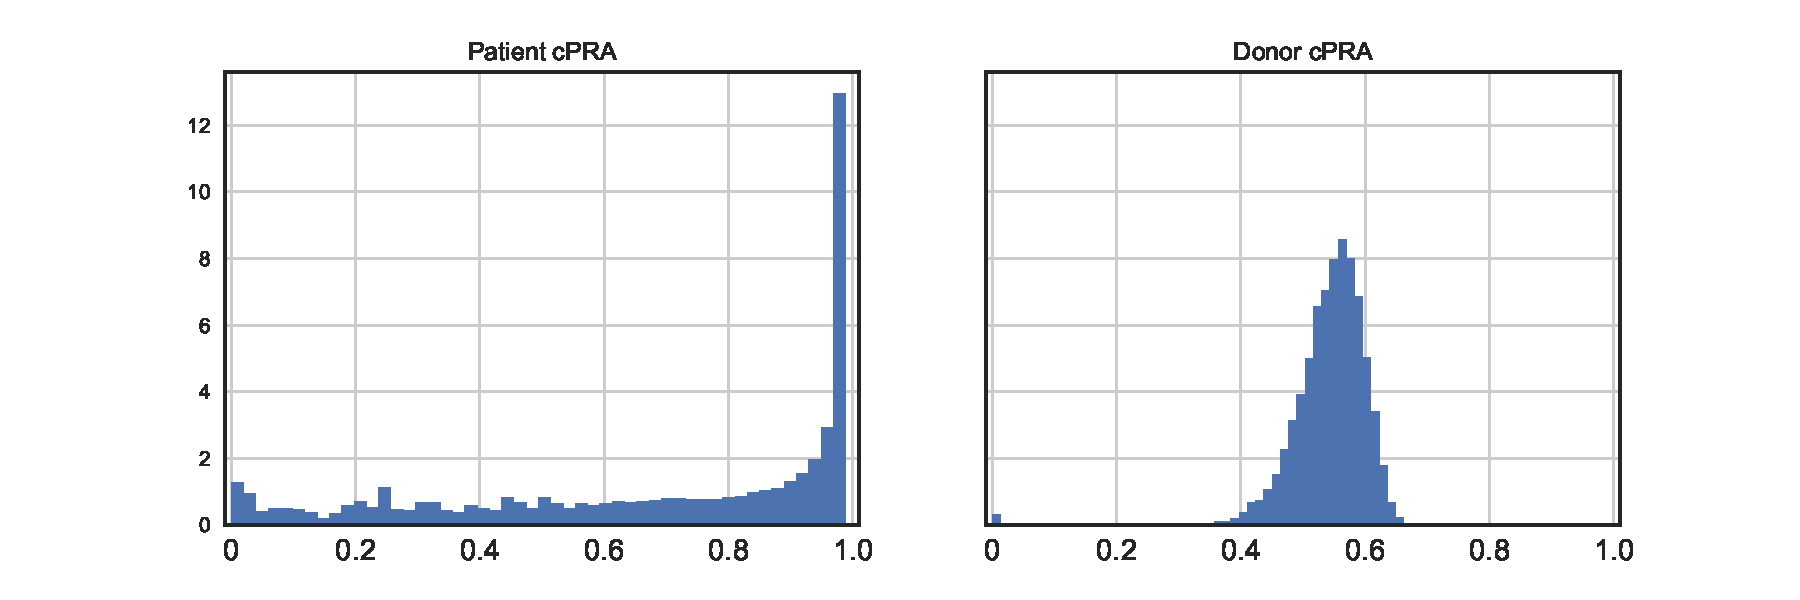
\includegraphics[width=1textwidth]{/Users/vitorhadad/Documents/kidney/matching/figures/computed_cpra.pdf}.
\caption{Computed patient and donor cPRA.}
\label{fig:cpra}
\end{figure}

\paragraph{Compatibility} A donor and a patient are deemed \emph{compatible} if they are blood-type compatible and tissue-type compatible. The latter is true when the donor's HLA profile exhibits no antigens that are unacceptable for the patient in any of the A, B, Bw, C, DR, DPB, DQ, and DQA loci.

\paragraph{Simulation} During a simulation, pairs are drawn from this artificial data set. Once a pair enters the pool, it immediately forms directed edges with existing compatible pairs.

\paragraph{Observable characteristics} For each pair, the agent observes the entry time, the waiting time, and 375 dummies corresponding to blood type and HLA profile of patient and donor. 




\subsection{Benchmarks}

In this work, we focus on maximizing the average number of matched pairs over $T$ periods, where $T$ is a large number relative to the rates of patient entry and death. 

\subsubsection{Myopic}

The \emph{myopic} algorithm finds the maximal number of matchings at every period, and clears it immediately. It disregards all observable characteristics of each pair, and in particular it disregards that some pairs might be useful to keep certain pairs may be easier or harder to match. In doing so, it may forgo the opportunity of matching a hard-to-match patient today, or postpone an easy-to-match pair for later.

\subsubsection{Infeasible Optimal (OPT)}

The infeasible optimal algorithm (henceforth OPT) does away with the uncertainty arising from the temporal structure of the problem: it knows exactly which pairs will come into the pool, as well as their arrival, and the duration of their sojourns. This algorithm is essentially a large static kidney matching problem, except that the set of available exchanges has the additional constraint that a cycle cannot exist between two vertices if their sojourns fail to overlap.

\subsubsection{Empirical comparison between myopic and OPT}

Figure \ref{}



 \begin{figure}
 \centering
 \hspace*{-4cm}
 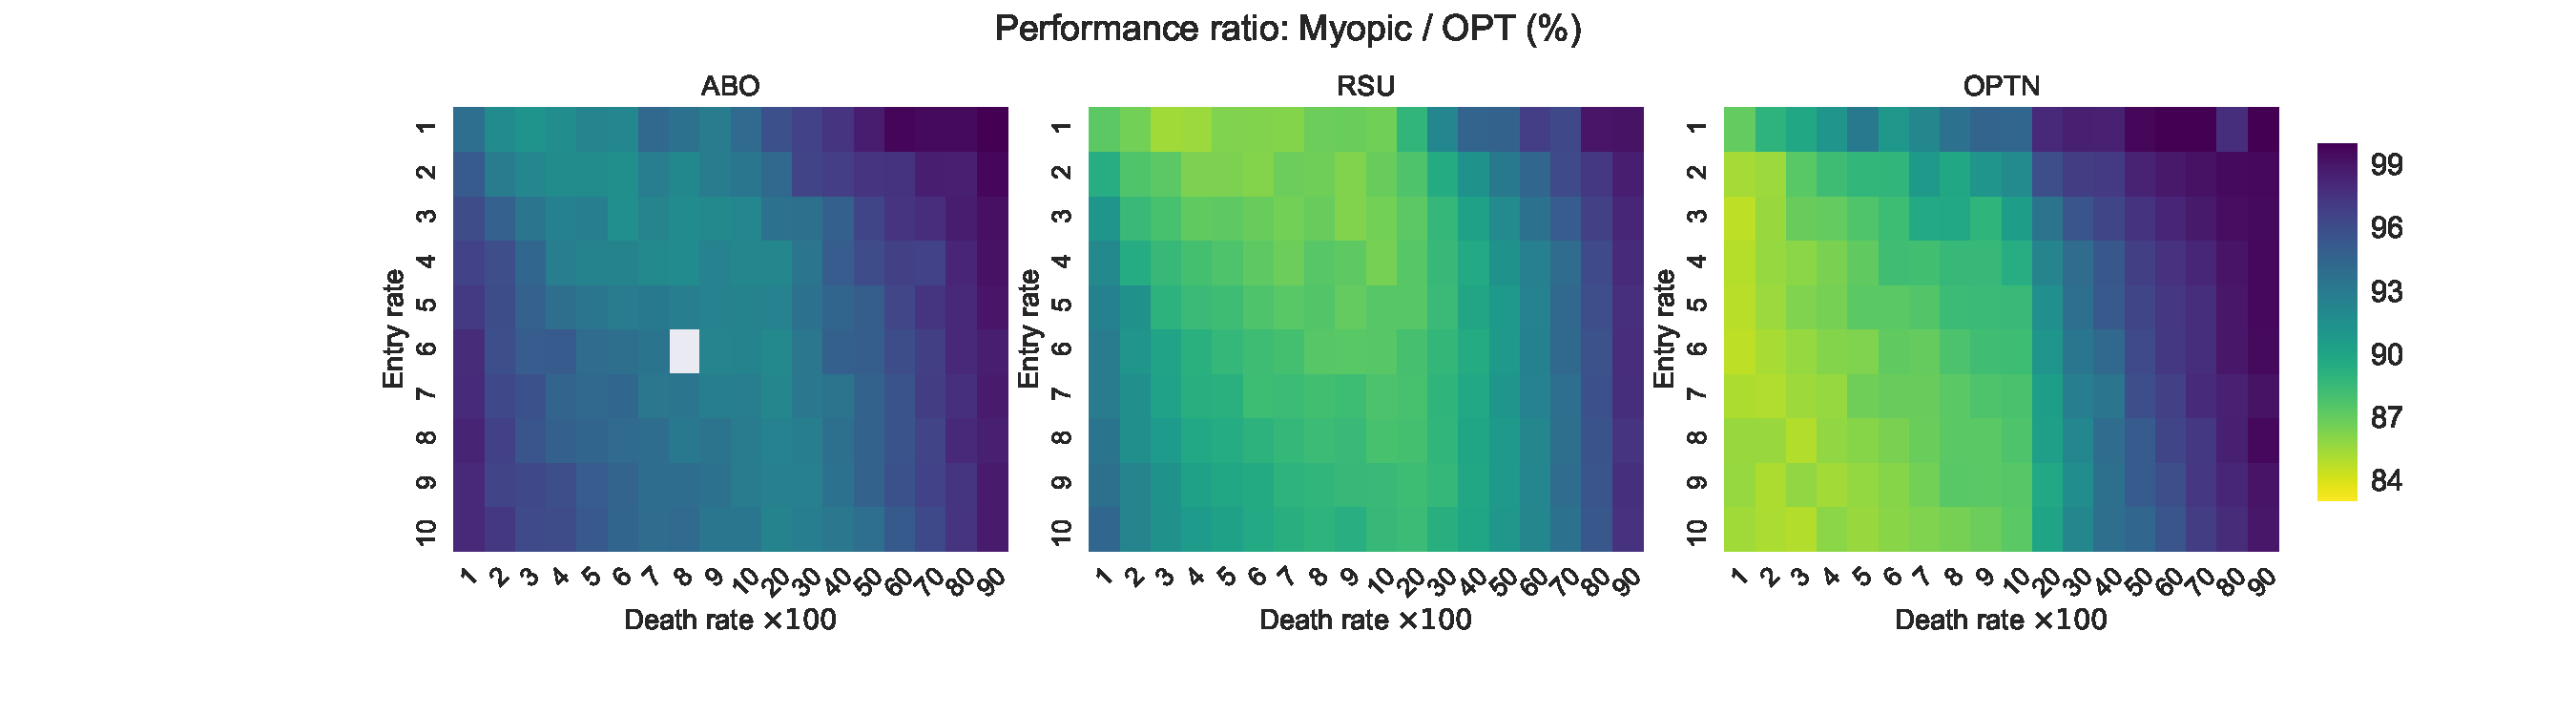
\includegraphics[width=1.5\textwidth]{/Users/vitorhadad/Documents/kidney/matching/phd_thesis/figures/greedy_opt_comparison_mcl2.pdf}
 \caption{\texttt{Myopic} matches roughly the same number of pairs per period as \texttt{OPT} when the death rate is high (moving rightwards on the graphs), or when entry rate is high (moving downwards on the graphs).}
 \label{fig:mab}
 \end{figure}



\subsection{Algorithms}

We divide our algorithms into three classes: \emph{direct prediction} methods, \emph{multi-armed bandit} methods and \emph{reinforcement learning} methods. They are explained next.

\subsubsection{Direct prediction} \label{subsubsec:direct_prediction}

Dynamic and static algorithms can split their work: the former can determine which pairs should be matched at each period, while the latter decides how they should be matched among themselves. The \emph{direct prediction} exploits this insight, essentially reducing the problem to a classification task: at each period, they aim to produce a 0-1 label for each node indicating whether is should be matched in this period (1) or left for later (0). Selected nodes are then passed to a static solver that finds the maximal matching among them. Once these nodes are cleared, time evolves to the next period. This is illustrated in Figure \ref{fig:direct_prediction}.

\begin{figure}
\centering
\hspace*{-1cm}
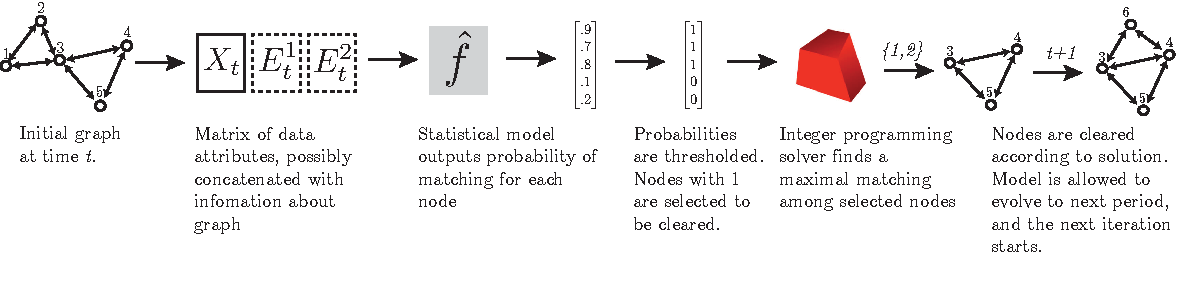
\includegraphics[width=1.1\textwidth]{/Users/vitorhadad/Documents/kidney/matching/phd_thesis/figures/direct_prediction.pdf}.
\caption{Direct prediction methods.}
\label{fig:direct_prediction}
\end{figure}

In order to produce data to feed into our ``classifier", each environment was simulated and solved using OPT, with each pair's observable characteristics as regressors, and a binary variable indicating whether they were matched or not. Each resulting artifical dataset of approximately 2 million observations was then fed to a series of predictive algorithms, including penalized logistic regression\cite{wu2009genome}, support vector machines with radial basis function kernels\cite{cortes1995support}, random forest classifiers\cite{breiman2001random}, gradient tree boosting classifiers\cite{friedman2001greedy} and deep feedforward networks\cite{goodfellow2016deep}. The performance of these algorithms as classification methods is compared in Table \ref{tab:direct_prediction}.

[[[The poor performance?? could be attributable to not having represented the data properly etc. Non-euclidean spaces big challenge etc]]]

 In order to represent information about the graph and how the nodes fit within it, we augment the original dataset using one or both of the following. First, with vertex properties for each node such as the number of in and out-edges, average neighbor degree, some centrality measures (betweenness, in-degree, out-degree, harmonic, closeness) and more exotic indices such as the core number and pagerank of each node\cite{newman2010networks}. Second, we augment the data using the \emph{node2vec} graph embedding algorithm of \cite{grover2016node2vec}, a continuous feature representation algorithm inspired by the skip-gram model.[[[More on this?]]]. These algorithms will produce auxiliary matrices $E_t^{1}$ and $E_t^2$ that are concatenated to the original data regressor matrix $X_t$, and the entire augmented data set can again be fed to the predictive algorithms above. Their performance is compared on the bottom half of Table \ref{tab:direct_prediction}.
 

 
 
\subsection{Multi-armed bandits}
 
We have access to the data-generating process (\emph{environments}) and an algorithm that is able to find the best matching for any data in hindsight (\texttt{OPT}). Therefore, in principle we could estimate the best choice of cycle to clear by simulating several periods ahead in the future, running \texttt{OPT}, and measuring the performance of our choice under any desired criterion. 

The approach outlined above turns out to be naive and incomplete, but it essentially contains the insight under which we will be working in this section. It is naive because simulations are computationally expensive, and in practice we cannot repeat them enough times get reliable estimates of the average performance for each cycle choice, especially in large graphs. It is also incomplete because it does not specify exactly what is the best information we should extract from \texttt{OPT} results. In order to solve the first problem, we leverage theory and algorithms from the multi-armed bandit (MAB) literature. For the second, we propose a secondary objective based on what we call \emph{pseudo-rewards}.

Our procedure is illustrated in Figures \ref{fig:mab} and \ref{fig:mab_step}. At the beginning of the period $t$, the agent receives a set of cycles $C$ that are available to be cleared. If $C$ is empty, nothing happens and we move to the next period. Otherwise, the agent then picks a cycle $c \in C$ and simulates the future, including new entries and deaths, up to a horizon $h$. Next, \texttt{OPT} is run twice, once normally, and once with the additional constraint that $c$ be removed today. The size of the resulting matching in these two scenarios is compared. Naturally, the constrained version of \texttt{OPT} cannot achieve anything better than its unconstrained counterpart, but it might get to be equal. If it is, the agent receives a \emph{pseudo-reward} of one, otherwise it receives zero. This process is repeated: at each iteration $\ell$, a cycle $c_{\ell}$ is chosen and its pseudo-reward $r_{c, \ell}$ is revealed. When a preset computational budget of $L(|C|)$ iterations is hit, the agent then analyses the whole history of cycle choices and pseudo-rewards $H_{t} = \{ (c_{\ell}, r_{c\ell} ) \}_{\ell=1}^{L}$, and decides whether to match one of the cycles or move on to the next period. If a cycle $c$ is chosen it is immediately cleared, however the environment does not evolve to the next period yet. Instead, the history $H_t$ is discarded the procedure is repeated again with a reduced set of actions $C' \subset C$ that produces a new history $H_t'$ and so on, until either there are no more available choices or the agent decides to allow the environment to move on to time $t+1$. When that at last happens, entries and deaths are revealed, the agent receives a new set of cycles, and the process begin anew. All past information is ignored.


Two important details were left out of the explanation above. First, how does the agent chooses the next cycle to test? Second, how does it decide which cycle to choose (or no cycle at all)? 


Let $c^{*}$ be a cycle that maximizes expected pseudo-rewards during one round of the algorithm:
$$c^{*} \in \arg\max_{c} E[r_{c\ell}] $$


 A \emph{multi-armed bandit} algorithm is a procedure to minimize \emph{regret} 


 \begin{figure}
 \centering
 \hspace*{-1cm}
 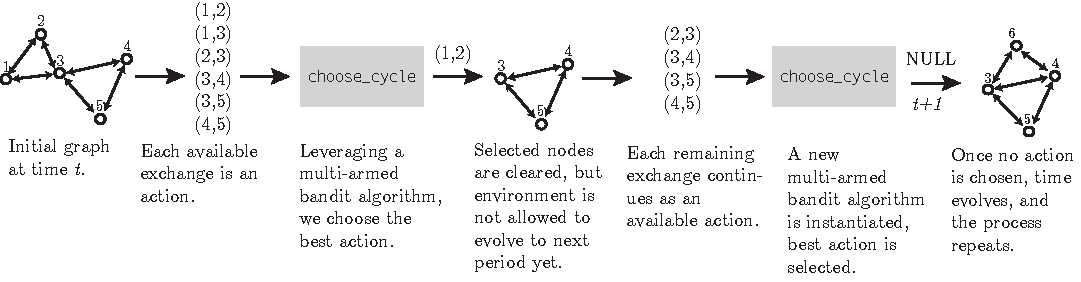
\includegraphics[width=1.1\textwidth]{/Users/vitorhadad/Documents/kidney/matching/phd_thesis/figures/mab.pdf}
 \caption{Multi-armed bandit methods.}
 \label{fig:mab}
 \end{figure}

 \begin{figure}
 \centering
 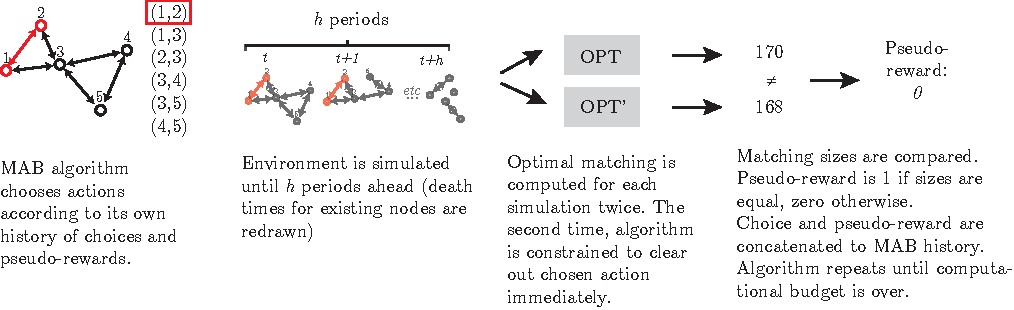
\includegraphics[width=1.1\textwidth]{/Users/vitorhadad/Documents/kidney/matching/phd_thesis/figures/mab_step.pdf}
 \caption{Pseudo-reward computation in one step of a multi-armed bandit algorithm.}
 \label{fig:mab_step}
 \end{figure}
 
  




% \subsection{Methods}
% 
% In this work, we propose a new kidney exchange algorithm that combines simulation-based search with a policy parametrized by neural networks. In the next paragraphs, we will explain each of these components in detail. However, first let us provide some motivation.
% 
% We begin by noting that we have a promising setup, as we are in possession of: good estimates of the data-generating process for each environment; an algorithm that is able to compute optimal actions, even if only in hindsight (\texttt{OPT}); one clear benchmark that we must beat (\texttt{Myopic}). At first glance, then, one might hypothesize that it would be possible to find reasonably good solutions using only simulations: simply simulate future states to a long horizon ahead, and choose today the action that on average leads to higher future rewards -- or the one that is most often chosen by \texttt{OPT}, or the one that most frequently leads to beating \texttt{Myopic}. Unfortunately, this turns out to be overly optimistic: approaches solely based on simulations do not perform very well, as shown in Table \ref{simulations_only}. We believe that the reason for this poor performance is the high branching factor of the problem -- in other words, there is high uncertainty about what the next period will look like.
% 
% 
% Reducing the problem:
% 
% 1. Our "actions" are simply a number of binary flags indicating who should be matched today and who should not
% 2. We can leverage the optimal algorithm to reduce the MDP to a simpler period-by-period MAB problem
% 3. Use 
% 
% % In lieu of just simulations, we propose to see each period's problem as a Bayesian multi-armed bandit problem (MAB). ... estimate... then use estimates as pseudo-counts... then sample from posterior.
% 
% 


%\insert{algo1.tex}

% Using Thompson sampling at each episode might sound like a greedy approach to a problem where current actions might have effects on future rewards, but here we *are* using future rewards since we can simulate the future \emph{and} also assume that we will be act optimally within a time horizon.


\section{Results} \label{sec:results}



\subsection{Short-run gains}

\section{Discussions and Extensions} \label{sec:discussion}

HLA mistmatch -- doctors are willing 

\section{Conclusion} \label{sec:conclusion}


\section{Acknowledgements}

This work was supported in part by Health Resources and Services Administration contract 234-2005-37011C. The content is the responsibility of the authors alone and does not necessarily reflect the views or policies of the Department of Health and Human Services, nor does mention of trade names, commercial products, or organizations imply endorsement by the U.S. Government.

\clearpage

\bibliographystyle{/Users/vitorhadad/Documents/kidney/matching/paper/te.bst}
\bibliography{references}


\clearpage

%\onehalfspacing

\section*{Tables} \label{sec:tab}
\addcontentsline{toc}{section}{Tables}



\clearpage

\section*{Figures} \label{sec:fig}
\addcontentsline{toc}{section}{Figures}




\clearpage

\section*{Appendix A. Placeholder} \label{sec:appendixa}
\addcontentsline{toc}{section}{Appendix A}



\end{document}